
\documentclass[tikz]{standalone}
\usepackage{graphicx}
\usepackage{lmodern}
\usepackage{import}
\usepackage{amsmath, amssymb, amsfonts}
\usetikzlibrary{calc}
\newcommand{\R}{\mathcal{R}}
\newcommand{\conscvx}{\mathrm{cons}_\mathrm{cvx}}
\newcommand{\Lcvx}{\mathcal{L}^{\mathrm{cvx}}}

\usetikzlibrary{arrows}

\begin{document}
	
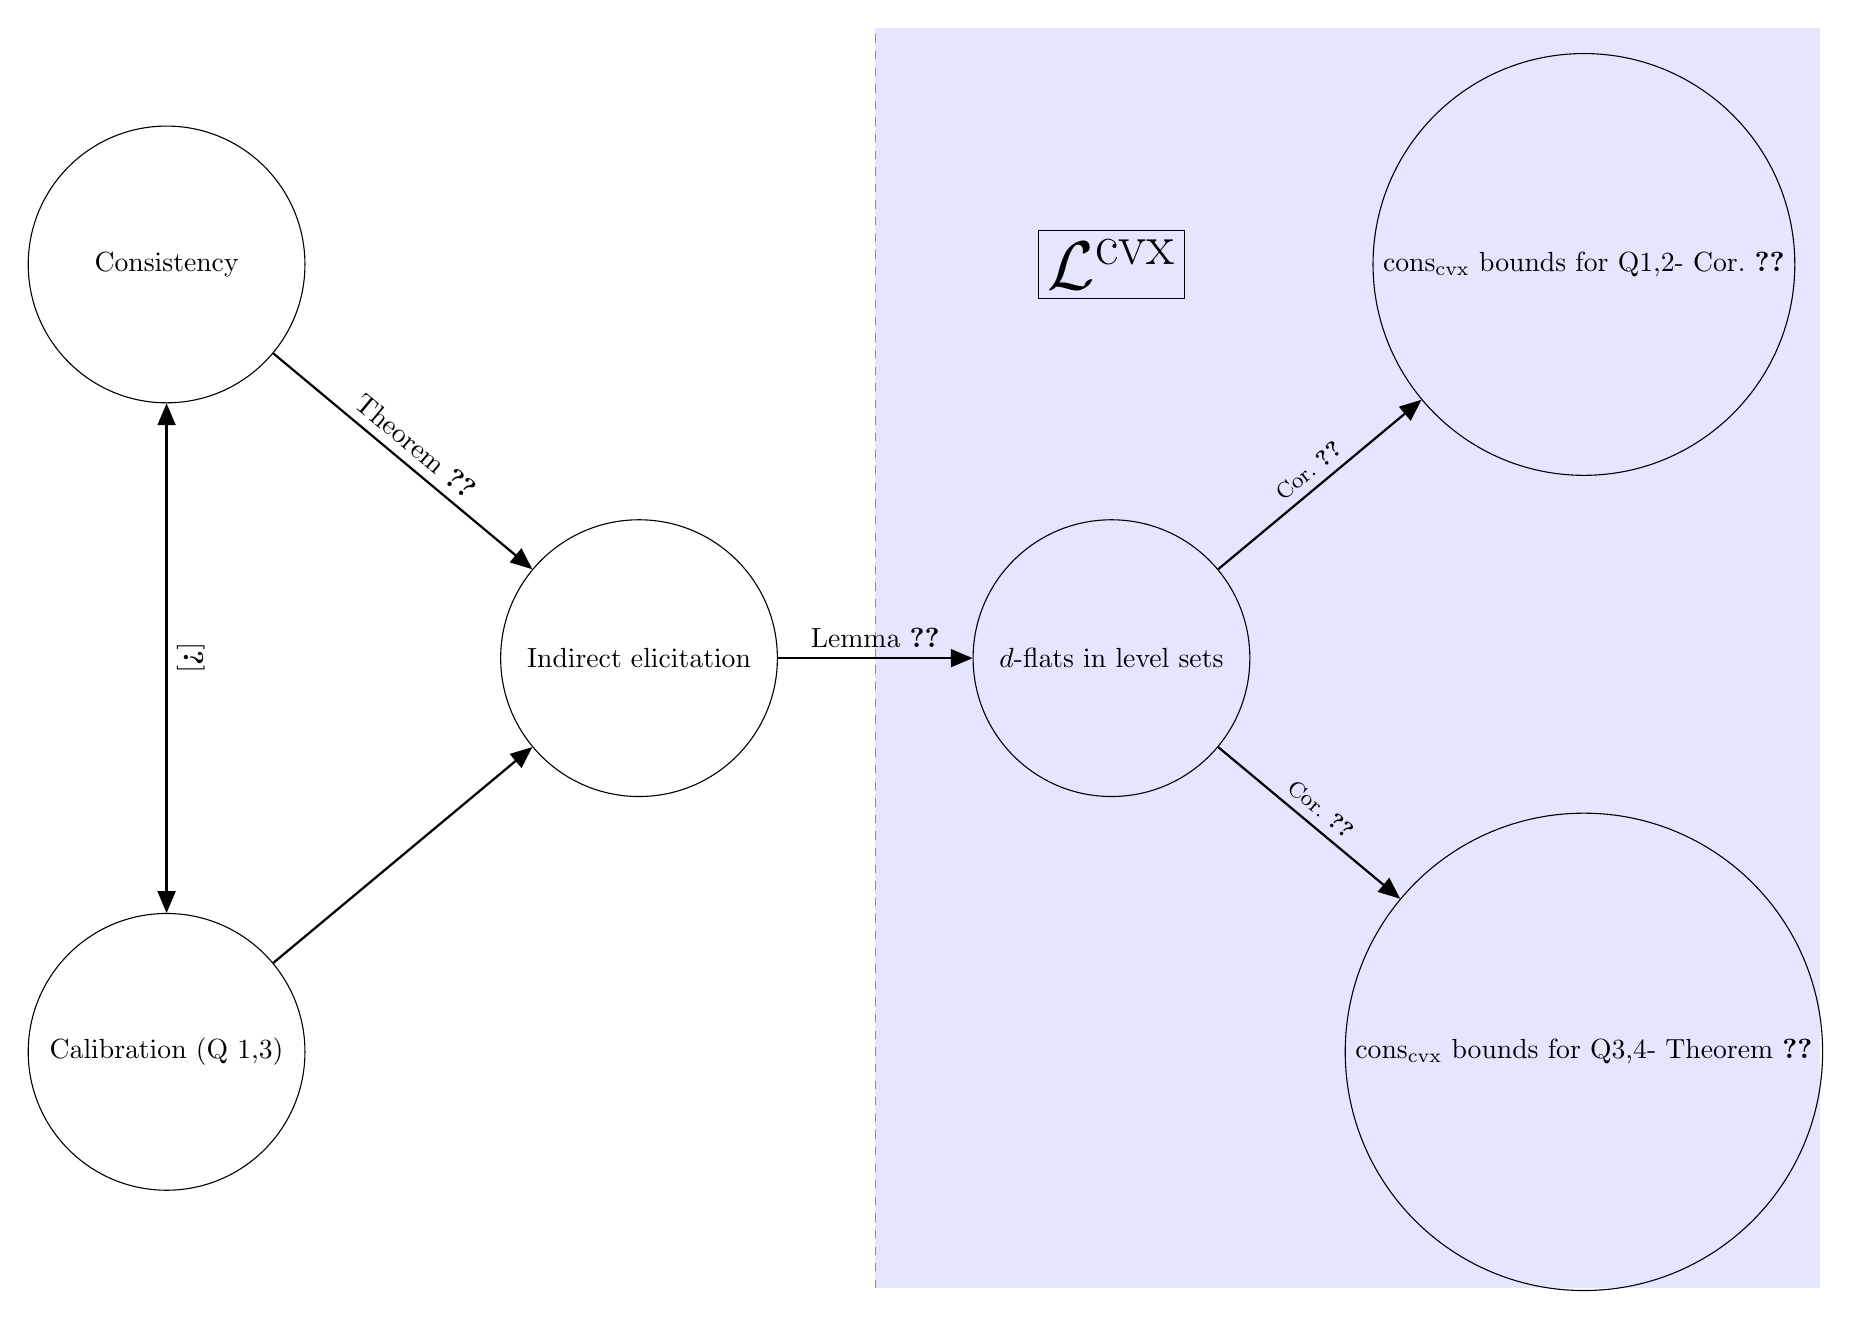
\begin{tikzpicture}

\tikzset{vertex/.style = {circle,draw,minimum width=10em}}
\tikzset{edge/.style = {->,> = triangle 45, thick}}
\tikzset{node/.style = {anchor=above, sloped}}

\path[fill=blue, fill opacity = 0.1] (0,-8) -- (0,8) -- (12,8) -- (12,-8) -- cycle;
\draw[dashed, opacity = 0.4] (0,-8) -- (0,8);
\node[draw] at (3,5) {{\Huge$\Lcvx$}};
%\draw (3,5)\node[above] {$\Lcvx$};

% vertices
\node[vertex] (consistent) at  (-9,5) {Consistency};
\node[vertex] (calibrated) at  (-9,-5) {Calibration (Q 1,3)};
\node[vertex] (indir-elic) at  (-3,0) {Indirect elicitation};


%\node[vertex] (consis-ell) at  (-4,2) {Consistency w.r.t. $\ell$};
%\node[vertex] (consis-gam) at  (2,2) {Consistency w.r.t. $\gamma$};

\node[vertex] (d-flats) at  (3,0) {$d$-flats in level sets};
%\node[vertex] (conscvx-bd) at (8,0) {$\conscvx(\gamma) \leq d$};
\node[vertex] (q1-bounds) at (9,5) {$\conscvx$ bounds for Q1,2- Cor.~\ref{ref}};
\node[vertex] (q4-bounds) at (9,-5) {$\conscvx$ bounds for Q3,4- Theorem~\ref{ref}};

%edges
\draw[edge, <->] (consistent) to node[above,sloped]{\cite{bartlett2006consistent}} (calibrated);
\draw[edge] (consistent) to node[above, sloped]{Theorem~\ref{thm:consistent-implies-indir-elic}} (indir-elic);
\draw[edge] (calibrated) to (indir-elic);
\draw[edge] (indir-elic) to node[above, sloped]{Lemma~\ref{lem:convex-flats-inf-dim}} (d-flats);

\draw[edge] (d-flats) to node[above, sloped]{{\footnotesize Cor.~\ref{cor:Pcodim-flat-elic-relint-prop}}} (q4-bounds);
\draw[edge] (d-flats) to node[above, sloped]{\footnotesize {Cor.~\ref{cor:Pcodim-flat-single-val-prop}}} (q1-bounds);
%\draw[edge] (conscvx-bd) to node[above, sloped]{\S~\ref{sec:finite-calib}} (q1-bounds);
%\draw[edge] (conscvx-bd) to node[above, sloped]{\S~\ref{sec:contin-consis}} (q4-bounds);

\end{tikzpicture}
	
\end{document}